\documentclass{lab1-article}

\title{Misure di focali}


\begin{document}


\begin{article}
\selectlanguage{italian}

\maketitle

\secsummary

Lo scopo dell'esperienza \`e la misura delle focali di una lente convergente
ed di una divergente.


\secmaterials

\begin{itemize}
\item Banco ottico con sorgente luminosa, schermo mobile e supporti per lenti;
\item cofanetto con un \emph{set} di lenti (convergenti e divergenti) di
  varie lunghezze focali;
\item metro a nastro (risoluzione 1~mm).
\end{itemize}


\secmeasurements

Per la legge delle lenti sottili, detta $p$ la distanza tra la sorgente e la
lente e $q$ la distanza tra la lente e l'immagine (a fuoco) si ha
\begin{align}
  \frac{1}{p} + \frac{1}{q} = \frac{1}{f},
\end{align}
dove $f$ \`e la distanza focale della lente.


\labsubsection{Lente convergente}

\begin{figure}[htb!]
\begin{center}
  \begin{tikzpicture}[scale=1.25]
    %\draw (0, 0) -- (1,1);
    \draw (0, 0) -- (6,0);
    \draw[->] (2, 0) -- (2,1);
    \draw[->] (2, 0) -- (2,-1);
    \draw [fill] (1.5,0) circle [radius=0.02];
    \draw [fill] (2.5,0) circle [radius=0.02];
    \draw[thick, ->] (1.25, 0) -- (1.25,0.5); % object
    \draw (1.25,0.5) -- (2, 0.5) -- (3.5, -1); %()
    \draw (1.25,0.5) -- (3.5, -1); %(2, 0)
    \draw[thick, ->] (3.5, 0) -- (3.5,-1); % image
    % notation
    \draw[<->] (1.25, -1.25) -- (2, -1.25); 
    \node [below] at (1.625,-1.25) {$p$};
    \draw[<->] (2, -1.25) -- (3.5,-1.25); 
    \node [below] at (2.75,-1.25) {$q$};
  \end{tikzpicture}
  \caption{Schema ottico per la lente convergente.}
  \label{fig:convergente}
\end{center}
\end{figure}

Si scelga una lente convergente dal cofanetto e si ponga sul banco ottico.
Fissata una distanza $p_i$ della lente dalla sorgente si sposti lo schermo
fino a che l'immagine non \`e a fuoco, e si misuri la corrispondente
distanza $q_i$. Si iteri il procedimento pi\`u volte (ad esempio 10), si
costruisca il grafico cartesiano di $(1/p_i,~1/q_i)$ e si esegua un \emph{fit}
lineare per determinare il potere diottrico della lente, che corrisponde
all'intercetta.

La misura della focale ottenuta \`e compatibile con il valore riportato sul
bordo della lente?

Si verifichi che il coefficiente angolare restituito dal \emph{fit}
sia compatibile con $-1$. Se ci\`o non fosse verificato, a cosa potremmo
ascrivere la discrepanza?


\labsubsection{Lente divergente}

Dato che la lente divergente non forma immagini reali, per questa misura
occorre anche una lente convergente \emph{di potere diottrico maggiore (in
modulo) rispetto a quello della divergente}. Possiamo considerare l'immagine
prodotta dalla lente convergente come una sorgente virtuale per la lente
divergente.

\begin{figure}[htb!]
\begin{center}
  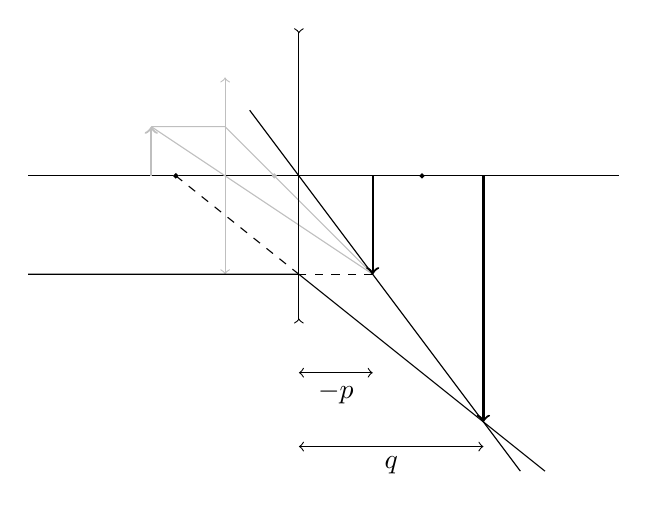
\begin{tikzpicture}[scale=1.25]
    %\draw (0, 0) -- (1,1);
    \draw (0, 0) -- (6,0);
    \draw[lightgray, ->] (2, 0) -- (2,1);
    \draw[lightgray,->] (2, 0) -- (2,-1);
    \draw [lightgray, fill] (1.5,0) circle [radius=0.02];
    \draw [lightgray, fill] (2.5,0) circle [radius=0.02];
    \draw[lightgray, thick, ->] (1.25, 0) -- (1.25,0.5); % old object
    \draw[lightgray] (1.25,0.5) -- (2, 0.5) -- (3.5, -1); 
    \draw[lightgray] (1.25,0.5) -- (3.5, -1); 
    \draw[thick, ->] (3.5, 0) -- (3.5,-1); % object (old image)
    % lens
    \draw[-<] (2.75, 0) -- (2.75,1.5);
    \draw[-<] (2.75, 0) -- (2.75,-1.5);
    \draw [fill] (4,0) circle [radius=0.02];
    \draw [fill] (1.5,0) circle [radius=0.02];
    % ray
    \draw[dashed] (3.5,-1) -- (2.75, -1); 
    \draw[dashed] (2.75,-1) -- (1.5, 0); 
    \draw (0,-1) -- (2.75, -1) -- (5.25, -3); 
    \draw (2.25, 2./3) -- (5., -3); 
    \draw[thick, ->] (15./8+2.75, 0) -- (15./8+2.75,-2.5); % image
    % notation
    \draw[<->] (2.75, -2.) -- (3.5, -2.); 
    \node [below] at (3.125,-2.) {$-p$};
    \draw[<->] (2.75, -2.75) -- (15./8+2.75,-2.75); 
    \node [below] at (3.69,-2.75) {$q$};

  \end{tikzpicture}
  \caption{Schema ottico per la lente divergente. 
    Notare che la sorgente per la lente divergente \`e virtuale.}
  \label{fig:divergente}
\end{center}
\end{figure}

In pratica: si ponga la lente convergente sul banco ottico e si metta a fuoco
l'immagine sullo schermo. A questo punto si posizioni la lente divergente
tra la convergente e lo schermo e si misuri la distanza $p_i$ (da prendere con
il segno negativo) tra la divergente e lo schermo stesso. Si allontani lo
schermo in modo da rimettere a fuoco l'immagine e si misuri la nuova distanza
$q_i$ (questa volta positiva) tra la divergente e lo schermo. Come nel caso
precedente, si iteri il procedimento pi\`u volte (ad esempio 10) e si stimi
il potere diottrico tramite un \emph{fit} lineare.
 

\secconsiderations

Quando si misura la distanza tra una lente ed una sorgente, potrebbe non essere
sufficiente prendere come errore la risoluzione del metro a nastro, in quanto
la posizione della lente nella ghiera di montaggio non \`e ben definita.
In altre parole la lente non \`e molto pi\`u sottile (e nemmeno pi\`u sottile)
della risoluzione del metro a nastro.

Quando si misura la distanza tra la lente e l'immagine, il contributo maggiore
all'errore di misura potrebbe essere dovuto alla messa a fuoco---pu\`o capitare
che l'immagine appaia a fuoco su un intervallo molto pi\`u grande del mm di
risoluzione del metro a nastro.


\end{article}
\end{document}
